\section{Analysis}
Our two basic research questions were addressed individually.

\subsection{Question 1}
To answer the first research question, we can rely on subjects' accuracy in distinguishing the two groups. We calculated this by combining the results for each as the distracter and the target. Then, we aggregated all the subjects and took the percentage that was correct. Our hypothesis was that participants can tell apart every group from every single group. To test this, we did a simple binomial t-test comparing participants' actual performance to chance ($\pi=0.5$). This method should have a tendency towards false negatives, as we are performing $136$ tests of significance. Nonetheless, using this paradigm, we found that $135/136$ tests were significant at the $p=0.05$ level.  

A significance test naturally can have some amount of false positives and false negatives. In our study, the most difficult for participants was the distinction between “p4m” and “pmm” (see Figure~\ref{pmmp4m} for an example). Interestingly, an expert given a small amount of time should have almost no trouble distinguishing them, as the lack of 4-fold rotation is quite obvious in "pmm." Across the 96 participants, only 56.8\% of trials were successful. On a single-tailed binomial distribution, there is a p-value of $0.06$ on that number of trials. While this misses the classical $0.05$ marker for significance, every single other group by group comparison meets it. Therefore, we find it likely that with more subjects, every group would have shown itself to be statistically distinguishable. The average accuracy fell right around 76.8\%, which is clearly far better than people would perform if they were mostly guessing. Further, due to the number of significance tests, there would be some natural variation in any specific test.

Technically, the data we collected were asymmetric; that is, we have separate data from when group $A$ serves as the target and group $B$ serves as the distracter than when group $A$ serves as the distracter and group $B$ serves as the target. See Figure~\ref{fullacc} for the non-symmetric accuracies. We performed a $\chi^2$ test for symmetry to determine the reasonability of otherwise lumping the data together. This McNemar's test failed standard tests for significance $p > 0.1$; however, it was close enough $p < 0.15$ that the possibility remains of some asymmetry. Nonetheless, for the purposes of this current experiment, the data was combined.

\begin{figure}[!ht]
\centering
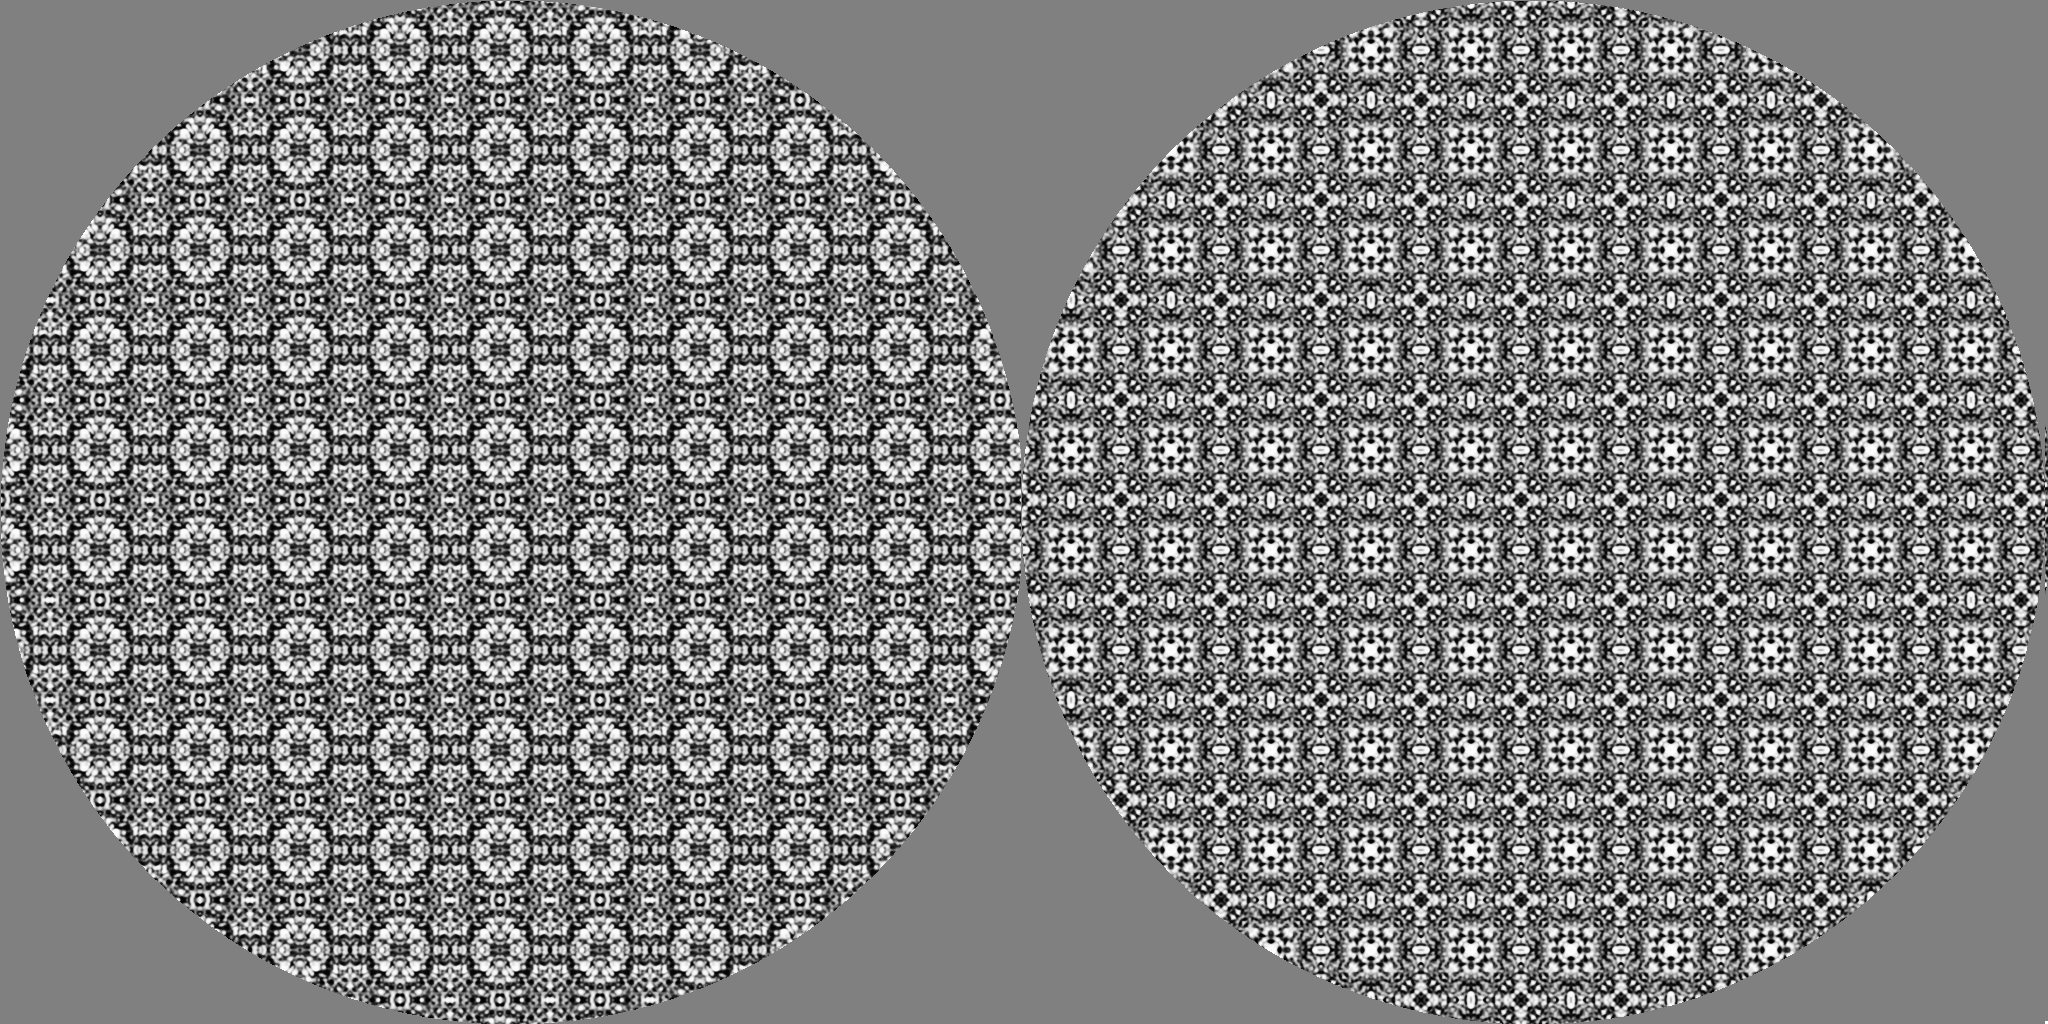
\includegraphics[width=0.9\columnwidth]{pmmp4m}
\label{pmmp4m}
\caption{PMM on the left (note the tiles lack reflection on the horizontal axis, but have it on the vertical axis), P4M on the right}
\end{figure}

\begin{figure}[!ht]
\centering
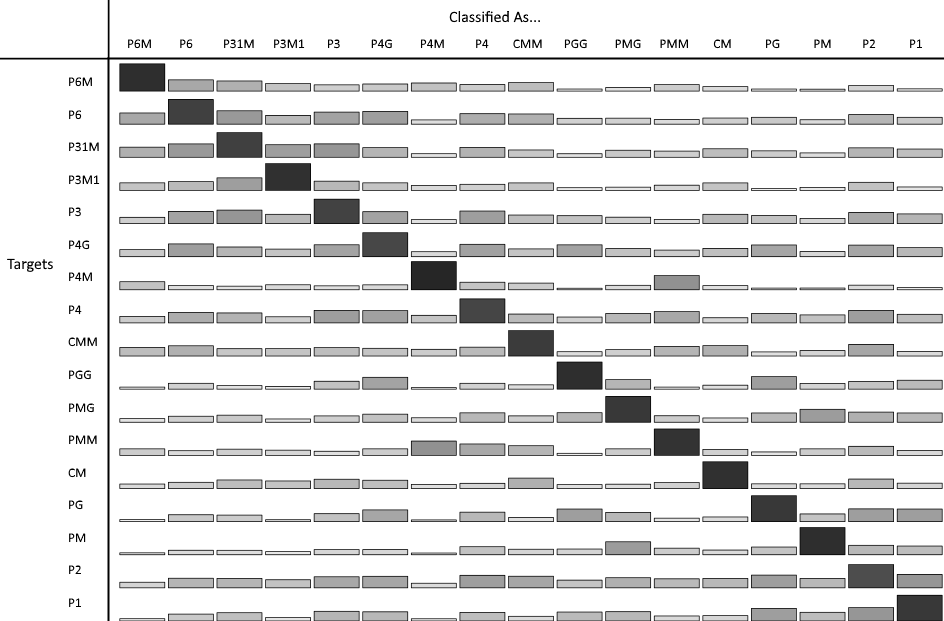
\includegraphics[width=0.9\columnwidth]{accuracies-grayscale}
\label{fullacc}
\caption{On the vertical we have the targets. On the top are the distracters. Main diagonal represents the aggregate accuracy in labeling that group correctly. The darker the bar, the closer to 1.0.}
\end{figure}

\subsection{Question 2}
To answer our second question, we used a Linear Mixed Effects Regression (GLMM) model. Since we wanted to predict what caused the subjects to choose correctly, we used accuracy as the response variable. Thus, the first step was to change each task to its own record. Then, each feature we considered could have a positive or negative impact on the accuracy.

Each task was boiled down to a comparison of the two symmetry group’s features. These features were whether or not the groups of the target and distracter images had the same tile shape, features determining whether the groups had the same value (Reflection, Glide Reflection, neither) along their reflection axes ($T_1, T_2, D_1, D_2$), and features for whether they had the same value (True or False) for 2-fold, 3-fold, 4-fold, and 6-fold rotation. Lastly, we also included the value for the shortest path (computed with Djikstra's algorithm) on the subgroup relation graph; for instance, the distance from “p6m” to “p6” is 1. While each of the first four refer to some basic feature of symmetry, the graph distance is included as an alternative theory. In short, it would posit that humans perceive symmetry very closely to its mathematical analysis, instead of as a collection of individual symmetries.

We used two random effect variables, which represent uncontrolled aspects of the model. The first is the actual participant who performed the task, which obviously has some effect on the accuracy. The second is the actual task they received: given that the target, goal, and distracter could each be in a different spot, there were two hundred possibilities for each of the 272 tasks. In early trials using a less random selection procedure, repeats of the same image in the same location were common enough to be noticeable by test participants. While we could have iteratively designed a uniform test set avoiding this issue, random effects allow us to control for the variance our methodology caused.

\begin{figure}[!ht]
\centering
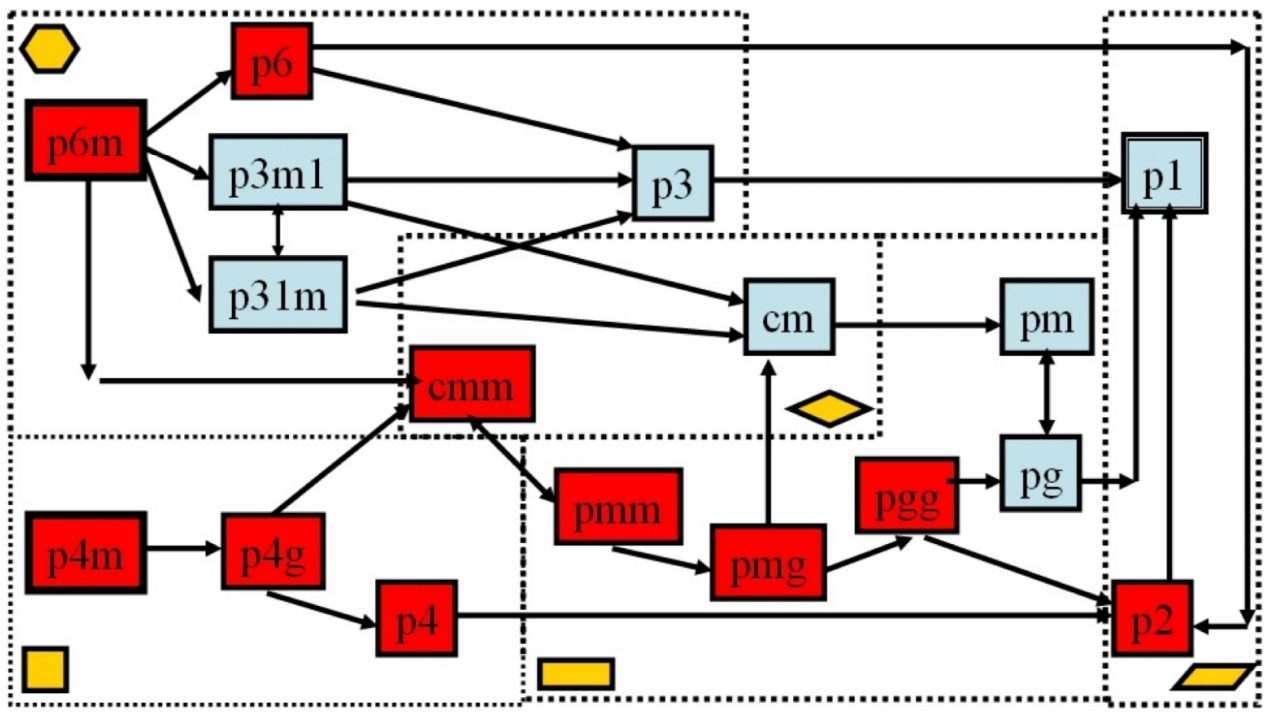
\includegraphics[width=0.9\columnwidth]{Yanxi_Graph}
\label{graph}
\caption{The subgroup relation graph}
\end{figure}

First, we performed a side-by-side model comparison, to determine which of the models had the lowest \textit{AIC}: a metric for evaluating models based on how well they explain the data given how many variables they include. We also looked at \textit{BIC}: a metric similar to the AIC that also takes sample size into account.  As we were looking at individual records, our sample size was quite high, at roughly 26,000. However, somewhat problematically in our case, BIC uses likelihood estimation that, to some extent, tacitly assumes the model could be correct, as it compares among possible models \citep{modelselect}\citep{techreport}. In our case, our data analysis explored variables relevant to symmetry and pattern recognition, but it could not possibly capture the entirety of the variance in human perception. Thus, while we report both, we focus on AIC as the more valid metric. Lastly, we used a pseudo-R-squared metric \citep{r2}. We report the conditional, rather than marginal, r-squared due to our lack of interest in exploring our random effects. We compared a rotation-based model, a reflection-based model, and a distance-based model. Results can be found in Table~\ref{results}. As can be seen, the model based on distance was the best naive model. 

\begin{table}
\centering
\begin{tabular}{|l|ccccc|}
\hline
& Rotation & Reflection & Distance & Best & All \\ \hline
AIC & 27251.1 &  27146.5 & 27105.8 & 26857.0 & 26856.3 \\ \hline
BIC & 27308.4 & 27203.7 & 27138.5 & 26922.4 & 26962.6 \\ \hline
$r^2$& 0.1234 & 0.1293 & 0.1317 & 0.1449 & 0.1454  \\ \hline
\end{tabular}
\label{results}
\caption{Comparison of theoretically-driven models}
\end{table}

Next, we found the best overall model from the pool of features described earlier. This model included distance, but additionally included the $T_1$ axis, which would correspond to bilateral reflection symmetry, the $D_1$ axis, which is the positive diagonal, along with 4-fold and 3-fold rotation. Finally, as a control case, we compared a model including all discussed features. All of these can be found in Table~\ref{results}.